\documentclass[a4paper, 11pt]{article}
\usepackage[UTF8, scheme = plain]{ctex}
\usepackage{xcolor}     %高亮使用的颜色
\usepackage{amsmath}
\usepackage{graphicx}
\usepackage{geometry}
\usepackage{listings}
\usepackage{textcomp}
\geometry{scale=0.8}
\linespread{1.5}
\usepackage{hyperref}

\title{	
\normalfont \normalsize
\textsc{School of Data and Computer Science, Sun Yat-sen University} \\ [25pt] %textsc small capital letters
\rule{\textwidth}{0.5pt} \\[0.4cm] % Thin top horizontal rule
\huge  E04 Futoshiki Puzzle (Forward Checking) \\ % The assignment title
\rule{\textwidth}{2pt} \\[0.5cm] % Thick bottom horizontal rule
\author{18308045 Zhengyang Gu}
\date{\normalsize September 21, 2020} 
}

\begin{document}
\maketitle
\tableofcontents
\newpage

\section{Futoshiki}
Futoshiki is a board-based puzzle game, also known under the name Unequal. It is playable on a square board having a given fixed size (4 × 4 for example).

The purpose of the game is to discover the digits hidden inside the board’s cells; each cell is filled with a digit between 1 and the board’s size. On each row and column each digit appears exactly once; therefore, when revealed, the digits of the board form a so-called Latin square.

At the beginning of the game some digits might be revealed. The board might also contain some inequalities between the board cells; these inequalities must be respected and can be used as clues in order to discover the remaining hidden digits.

Each puzzle is guaranteed to have a solution and only one.

You can play this game online: http://www.futoshiki.org/.


\section{Tasks}
\begin{enumerate}

\item  Please solve the above Futoshiki puzzle ( Figure 1 ) with forward checking algorithm.

\item  Write the related codes and take a screenshot of the running results in the file named E04 YourNumber.pdf, and send it to ai 2018@foxmail.com.

\end{enumerate}

\section{Codes}
\definecolor{mygreen}{rgb}{0,0.6,0}
\definecolor{mygray}{rgb}{0.5,0.5,0.5}
\definecolor{mymauve}{rgb}{0.58,0,0.82}
\lstset{
    backgroundcolor=\color{lightgray}, 
    basicstyle = \footnotesize,       
    breakatwhitespace = false,        
    breaklines = true,                 
    captionpos = b,                    
    commentstyle = \color{mygreen}\bfseries,
    extendedchars = false,             
    frame =shadowbox, 
    framerule=0.5pt,
    keepspaces=true,
    keywordstyle=\color{blue}\bfseries, % keyword style
    language = C++,                     % the language of code
    otherkeywords={string}, 
    numbers=left, 
    numbersep=5pt,
    numberstyle=\tiny\color{mygray},
    rulecolor=\color{black},         
    showspaces=false,  
    showstringspaces=false, 
    showtabs=false,    
    stepnumber=1,         
    stringstyle=\color{mymauve},        % string literal style
    tabsize=2,          
    title=\lstname                      
}
\begin{lstlisting}
//
// Created by GreenArrow on 2020/9/14.
//

#include <cstring>
#include <ctime>
#include <iostream>
#include <vector>

using namespace std;

struct my_tuple
{
    int x;
    int y;
    int value;
};

class FutoshikiPuzzle
{
public:
    vector<vector<int>> maps;
    vector<pair<pair<int, int>, pair<int, int>>> less_constraints;
    int nRow, nColumn;
    //表示第x行中某个数字是否存在
    int Count_RowNumbers[9][10];
    //表示第y列某个数字是否存在
    int Count_ColumnNumbers[9][10];
    int total = 0;
    //表示(x,y)点value值是否因FC被剪枝
    unsigned char is_pruned[9][9][10];
    //表示(x,y)点被剪枝的个数
    unsigned char pruned_num[9][9];
    vector<my_tuple> restore;

    void initial()
    {
        //初始地图
        maps = {{0, 0, 0, 7, 3, 8, 0, 5, 0},
                {0, 0, 7, 0, 0, 2, 0, 0, 0},
                {0, 0, 0, 0, 0, 9, 0, 0, 0},
                {0, 0, 0, 4, 0, 0, 0, 0, 0},
                {0, 0, 1, 0, 0, 0, 6, 4, 0},
                {0, 0, 0, 0, 0, 0, 2, 0, 0},
                {0, 0, 0, 0, 0, 0, 0, 0, 0},
                {0, 0, 0, 0, 0, 0, 0, 0, 0},
                {0, 0, 0, 0, 0, 0, 0, 0, 6}};
        nRow = maps.size();
        nColumn = maps[0].size();

        //添加限制
        addConstraints(0, 0, 0, 1);
        addConstraints(0, 3, 0, 2);
        addConstraints(1, 3, 1, 4);
        addConstraints(1, 6, 1, 7);
        addConstraints(2, 6, 1, 6);
        addConstraints(2, 1, 2, 0);
        addConstraints(2, 2, 2, 3);
        addConstraints(2, 3, 3, 3);
        addConstraints(3, 3, 3, 2);
        addConstraints(3, 5, 3, 4);
        addConstraints(3, 5, 3, 6);
        addConstraints(3, 8, 3, 7);
        addConstraints(4, 1, 3, 1);
        addConstraints(4, 5, 3, 5);
        addConstraints(4, 0, 4, 1);
        addConstraints(5, 4, 4, 4);
        addConstraints(5, 8, 4, 8);
        addConstraints(5, 1, 5, 2);
        addConstraints(5, 4, 5, 5);
        addConstraints(5, 7, 5, 6);
        addConstraints(5, 1, 6, 1);
        addConstraints(6, 6, 5, 6);
        addConstraints(6, 8, 5, 8);
        addConstraints(6, 3, 6, 4);
        addConstraints(7, 7, 6, 7);
        addConstraints(7, 1, 8, 1);
        addConstraints(8, 2, 7, 2);
        addConstraints(7, 5, 8, 5);
        addConstraints(8, 8, 7, 8);
        addConstraints(8, 5, 8, 6);

        //初始化域
        memset(is_pruned, 0, sizeof(is_pruned));
        for (int x = 0; x < 9; x++)
        {
            for (int y = 0; y < 9; y++)
            {
                int i = maps[x][y];
                if (i)
                {
                    Count_RowNumbers[x][i]++;
                    Count_ColumnNumbers[y][i]++;
                    for (int row_or_col = 0; row_or_col < 9; row_or_col++)
                    {
                        if (row_or_col != x)
                        {
                            if (!is_pruned[row_or_col][y][i])
                            {
                                is_pruned[row_or_col][y][i] = 1;
                                pruned_num[row_or_col][y]++;
                            }
                        }
                        if (row_or_col != y)
                        {
                            if (!is_pruned[x][row_or_col][i])
                            {
                                is_pruned[x][row_or_col][i] = 1;
                                pruned_num[x][row_or_col]++;
                            }
                        }
                    }
                }
            }
        }
        for (auto &less_constraint : less_constraints)
        {
            int x1 = less_constraint.first.first;
            int y1 = less_constraint.first.second;
            int x2 = less_constraint.second.first;
            int y2 = less_constraint.second.second;
            int value1 = maps[x1][y1];
            int value2 = maps[x2][y2];
            if (value1 && !value2)
            {
                for (int value = 1; value <= value1; value++)
                {
                    if (!is_pruned[x2][y2][value])
                    {
                        is_pruned[x2][y2][value] = 1;
                        pruned_num[x2][y2]++;
                    }
                }
            }
            else if (!value1 && value2)
            {
                for (int value = value2; value <= 9; value++)
                {
                    if (!is_pruned[x1][y1][value])
                    {
                        is_pruned[x1][y1][value] = 1;
                        pruned_num[x1][y1]++;
                    }
                }
            }
        }
        return;
    }

    void addConstraints(int x, int y, int x1, int y1)
    {
        less_constraints.push_back({{x, y},
                                    {x1, y1}});
    }

    //检查当前位置是否可行
    bool check(int x, int y)
    {
        for (int i = 1; i < 10; i++)
        {
            if (Count_RowNumbers[x][i] > 1 || Count_ColumnNumbers[y][i] > 1)
            {
                return false;
            }
        }

        for (auto &less_constraint : less_constraints)
        {
            if (less_constraint.first.first == x && less_constraint.first.second == y)
            {
                if (maps[x][y] == 9)
                {
                    return false;
                }
                if (maps[less_constraint.second.first][less_constraint.second.second] > 0 &&
                    maps[less_constraint.second.first][less_constraint.second.second] <= maps[x][y])
                {
                    return false;
                }
            }
        }

        for (auto &less_constraint : less_constraints)
        {
            if (less_constraint.second.first == x && less_constraint.second.second == y)
            {
                if (maps[x][y] == 1)
                {

                    return false;
                }
                if (maps[less_constraint.first.first][less_constraint.first.second] > 0 &&
                    maps[less_constraint.first.first][less_constraint.first.second] >= maps[x][y])
                {

                    return false;
                }
            }
        }
        return true;
    }

    //显示图片
    void show()
    {
        for (int i = 0; i < nRow; i++)
        {
            for (int j = 0; j < nColumn; j++)
            {
                cout << maps[i][j] << " ";
            }
            cout << endl;
        }
        cout << "======================" << endl;
    }

    void find_next(int &next_x, int &next_y)
    {
        for (next_x = 0; next_x < 9; next_x++)
        {
            for (next_y = 0; next_y < 9; next_y++)
            {
                if (!maps[next_x][next_y])
                {
                    goto next;
                }
            }
        }
    next:
        int temp_x, temp_y;
        for (temp_x = next_x, temp_y = next_y + 1; temp_y < 9; temp_y++)
        {
            if (!maps[temp_x][temp_y] && pruned_num[next_x][next_y] < pruned_num[temp_x][temp_y])
            {
                next_y = temp_y;
            }
        }
        for (temp_x = next_x + 1; temp_x < 9; temp_x++)
        {
            for (temp_y = 0; temp_y < 9; temp_y++)
            {
                if (!maps[temp_x][temp_y] && pruned_num[next_x][next_y] < pruned_num[temp_x][temp_y])
                {
                    next_x = temp_x;
                    next_y = temp_y;
                }
            }
        }
    }

    bool search(int x, int y)
    {
        if (maps[x][y] == 0)
        {
        	total++;
            for (int i = 1; i < 10; i++)
            {
                maps[x][y] = i;
                Count_RowNumbers[x][i]++;
                Count_ColumnNumbers[y][i]++;
                if (check(x, y))
                {
                    if (x == 8 && y == 8)
                    {
                        return true;
                    }
                    int next_x, next_y;
                    if (y != 8)
                    {
                        next_x = x;
                        next_y = y + 1;
                    }
                    else
                    {
                        next_x = x + 1;
                        next_y = 0;
                    }

                    if (search(next_x, next_y))
                    {
                        return true;
                    }
                }
                maps[x][y] = 0;
                Count_RowNumbers[x][i]--;
                Count_ColumnNumbers[y][i]--;
            }
        }
        else
        {
            if (x == 8 && y == 8)
            {
                return true;
            }
            int next_x, next_y;
            if (y != 8)
            {
                next_x = x;
                next_y = y + 1;
            }
            else
            {
                next_x = x + 1;
                next_y = 0;
            }

            if (search(next_x, next_y))
            {
                return true;
            }
        }
        return false;
    }

    bool FC_search(int x, int y)
	{
		total++;
		my_tuple back;
		for (int i = 1; i < 10; i++)
		{
			if (!is_pruned[x][y][i])
			{
				maps[x][y] = i;
				Count_RowNumbers[x][i]++;
				Count_ColumnNumbers[y][i]++;
				if (check(x, y))
				{
					int restore_num = 0;
					for (int row_or_col = 0; row_or_col < 9; row_or_col++)
					{
						if (!maps[row_or_col][y] && !is_pruned[row_or_col][y][i])
						{
							is_pruned[row_or_col][y][i] = 1;
							pruned_num[row_or_col][y]++;
							restore.push_back({row_or_col, y, i});
							restore_num++;
						}
						if (!maps[x][row_or_col] && !is_pruned[x][row_or_col][i])
						{
							is_pruned[x][row_or_col][i] = 1;
							pruned_num[x][row_or_col]++;
							restore.push_back({x, row_or_col, i});
							restore_num++;
						}
					}
					for (auto &less_constraint : less_constraints)
					{
						int x1 = less_constraint.first.first;
						int y1 = less_constraint.first.second;
						int x2 = less_constraint.second.first;
						int y2 = less_constraint.second.second;
						if (x1 == x && y1 == y)
						{
							if (!maps[x2][y2])
							{
								for (int value = 1; value <= i; value++)
								{
									if (!is_pruned[x2][y2][value])
									{
										is_pruned[x2][y2][value] = 1;
										pruned_num[x2][y2]++;
										restore.push_back({x2, y2, value});
										restore_num++;
									}
								}
							}
						}
						if (x2 == x && y2 == y)
						{
							if (!maps[x1][y1])
							{
								for (int value = i; value <= 9; value++)
								{
									if (!is_pruned[x1][y1][value])
									{
										is_pruned[x1][y1][value] = 1;
										pruned_num[x1][y1]++;
										restore.push_back({x1, y1, value});
										restore_num++;
									}
								}
							}
						}
					}
					int next_x, next_y;
					find_next(next_x, next_y);
					if (next_x == 9)
					{
						return true;
					}
					if (FC_search(next_x, next_y))
					{
						return true;
					}
					while (restore_num--)
					{
						back = restore.back();
						is_pruned[back.x][back.y][back.value] = 0;
						pruned_num[back.x][back.y]--;
						restore.pop_back();
					}
				}
			}
			maps[x][y] = 0;
			Count_RowNumbers[x][i]--;
			Count_ColumnNumbers[y][i]--;
		}
		return false;
	}
};

int main()
{
    FutoshikiPuzzle *futoshikiPuzzle = new FutoshikiPuzzle();
    futoshikiPuzzle->initial();
    futoshikiPuzzle->show();
    clock_t start = clock();
    futoshikiPuzzle->search(0, 0);
    clock_t end = clock();
    double endtime = (double)(end - start) / CLOCKS_PER_SEC;
    cout << "无FC:" << endl;
    futoshikiPuzzle->show();
    cout << "时间:" << endtime << " s" << endl;
    cout << "search数:" << futoshikiPuzzle->total << endl;
    delete futoshikiPuzzle;
    futoshikiPuzzle = new FutoshikiPuzzle();
    futoshikiPuzzle->initial();
	int next_x, next_y;
	futoshikiPuzzle->find_next(next_x, next_y);
    start = clock();
    futoshikiPuzzle->FC_search(next_x, next_y);
    end = clock();
    endtime = (double)(end - start) / CLOCKS_PER_SEC;
    cout << "有FC:" << endl;
    futoshikiPuzzle->show();
    cout << "时间:" << endtime << " s" << endl;
    cout << "search数:" << futoshikiPuzzle->total << endl;
}
\end{lstlisting}

\section{Results}
\begin{figure}[ht]
	\centering
	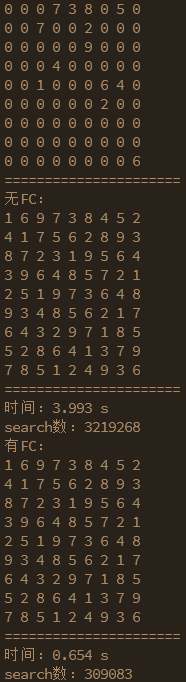
\includegraphics[width=7cm]{result.png}
	\caption{result}
\end{figure}


%\clearpage
%\bibliography{E:/Papers/LiuLab}
%\bibliographystyle{apalike}
\end{document} 
%%% Local Variables:
%%% mode: latex
%%% TeX-master: t
%%% End: